% THIS IS SIGPROC-SP.TEX - VERSION 3.1
% WORKS WITH V3.2SP OF ACM_PROC_ARTICLE-SP.CLS
% APRIL 2009
%
% It is an example file showing how to use the 'acm_proc_article-sp.cls' V3.2SP
% LaTeX2e document class file for Conference Proceedings submissions.
% ----------------------------------------------------------------------------------------------------------------
% This .tex file (and associated .cls V3.2SP) *DOES NOT* produce:
%       1) The Permission Statement
%       2) The Conference (location) Info information
%       3) The Copyright Line with ACM data
%       4) Page numbering
% ---------------------------------------------------------------------------------------------------------------
% It is an example which *does* use the .bib file (from which the .bbl file
% is produced).
% REMEMBER HOWEVER: After having produced the .bbl file,
% and prior to final submission,
% you need to 'insert'  your .bbl file into your source .tex file so as to provide
% ONE 'self-contained' source file.
%
% Questions regarding SIGS should be sent to
% Adrienne Griscti ---> griscti@acm.org
%
% Questions/suggestions regarding the guidelines, .tex and .cls files, etc. to
% Gerald Murray ---> murray@hq.acm.org
%
% For tracking purposes - this is V3.1SP - APRIL 2009

\documentclass{acm_proc_article-sp}
\usepackage{enumitem}
\usepackage{graphicx}
\begin{document}

\title{Finding Similar Questions from Community-based QA Services}
%
% You need the command \numberofauthors to handle the 'placement
% and alignment' of the authors beneath the title.
%
% For aesthetic reasons, we recommend 'three authors at a time'
% i.e. three 'name/affiliation blocks' be placed beneath the title.
%
% NOTE: You are NOT restricted in how many 'rows' of
% "name/affiliations" may appear. We just ask that you restrict
% the number of 'columns' to three.
%
% Because of the available 'opening page real-estate'
% we ask you to refrain from putting more than six authors
% (two rows with three columns) beneath the article title.
% More than six makes the first-page appear very cluttered indeed.
%
% Use the \alignauthor commands to handle the names
% and affiliations for an 'aesthetic maximum' of six authors.
% Add names, affiliations, addresses for
% the seventh etc. author(s) as the argument for the
% \additionalauthors command.
% These 'additional authors' will be output/set for you
% without further effort on your part as the last section in
% the body of your article BEFORE References or any Appendices.

\numberofauthors{3} %  in this sample file, there are a *total*
% of EIGHT authors. SIX appear on the 'first-page' (for formatting
% reasons) and the remaining two appear in the \additionalauthors section.
%
\author{
% You can go ahead and credit any number of authors here,
% e.g. one 'row of three' or two rows (consisting of one row of three
% and a second row of one, two or three).
%
% The command \alignauthor (no curly braces needed) should
% precede each author name, affiliation/snail-mail address and
% e-mail address. Additionally, tag each line of
% affiliation/address with \affaddr, and tag the
% e-mail address with \email.
%
% 1st. author
\alignauthor
Stephanie Valentine\\
       \affaddr{Department of Computer Science and Engineering}\\
       \affaddr{College Station, Texas}\\
       \email{valentine@cs.tamu.edu}
% 2nd. author
\alignauthor
Shiqiang Guo\\
     \affaddr{Department of Computer Science and Engineering}\\
     \affaddr{College Station, Texas}\\
     \email{pkushiqian@neo.tamu.edu}
% 3rd. author
\alignauthor 
Jung In Koh\\
      \affaddr{Department of Computer Science and Engineering}\\
      \affaddr{College Station, Texas}\\
      \email{jungin@neo.tamu.edu}
% use '\and' if you need 'another row' of author names
}
% There's nothing stopping you putting the seventh, eighth, etc.
% author on the opening page (as the 'third row') but we ask,
% for aesthetic reasons that you place these 'additional authors'
% in the \additional authors block, viz.
%\additionalauthors{Additional authors: John Smith (The Th{\o}rv{\"a}ld Group,
%email: {\texttt{jsmith@affiliation.org}}) and Julius P.~Kumquat
%(The Kumquat Consortium, email: {\texttt{jpkumquat@consortium.net}}).}
%\date{30 July 1999}
% Just remember to make sure that the TOTAL number of authors
% is the number that will appear on the first page PLUS the
% number that will appear in the \additionalauthors section.

\maketitle
\begin{abstract}
This paper provides a sample of a \LaTeX\ document which conforms to
the formatting guidelines for ACM SIG Proceedings.
It complements the document \textit{Author's Guide to Preparing
ACM SIG Proceedings Using \LaTeX$2_\epsilon$\ and Bib\TeX}. This
source file has been written with the intention of being
compiled under \LaTeX$2_\epsilon$\ and BibTeX.

The developers have tried to include every imaginable sort
of ``bells and whistles", such as a subtitle, footnotes on
title, subtitle and authors, as well as in the text, and
every optional component (e.g. Acknowledgments, Additional
Authors, Appendices), not to mention examples of
equations, theorems, tables and figures.

To make best use of this sample document, run it through \LaTeX\
and BibTeX, and compare this source code with the printed
output produced by the dvi file.
\end{abstract}

% A category with the (minimum) three required fields
\category{H.4}{Information Systems Applications}{Miscellaneous}
%A category including the fourth, optional field follows...
\category{D.2.8}{Software Engineering}{Metrics}[complexity measures, performance measures]

\terms{Theory}

\keywords{ACM proceedings, \LaTeX, text tagging} % NOT required for Proceedings

\section{Introduction}
Traditionally people found knowledge in books, the classroom or by asking anyone they could reach. With the recent popularity of web-based community question and answer (CQA) sites, like Yahoo Answers, Stackoverflow.com, Quora etc., people now frequently use these channels to ask their questions, especially in technical areas. Often, however, the question a user wants to post has been posted before. Most CQA websites ask users to search a question before posting it, with the idea that if a user could find similar questions, they can get the answer immediately without waiting for someone to answer their question. However, searching for similar questions is not trivial. Even if two questions have the same meaning, they could appear in totally different way.  For example, ``How can I express a for loop in Python?" and ``Is there any way to iterate through a range of integers?" are two similar questions, but they neither share many common words nor follow identical syntactic structure. 

Much work has been done regarding this topic, but most involve quite simple ideas buried deep within a complex system. In this project, we decouple the simple ideas from the complex systems and compare them against one another in a single system. We used a bag-of-words vector model and cosine as our similarity measure. We formed the vectors according to the simple ideas recommended by other researchers. These vectorizers modify the original document (baseline TFIDF) by: adding synonyms, increasing weight of nouns and verbs, and adding N-gram (phrases of length N). The goal of this work is to test the validity and comparative benefits of these ideas.

We collected data from two sources to form three datasets with which to test our system. One dataset is composed of questions from StackOverflow.com with the tag ``Python". A second dataset is composed of questions from English.Stack
Exchange.com. 
The third dataset combines the English and Python datasets into a single, multi-domain dataset.


\section{Related Works}
A batch of research has been done on this topic. The relative original work was published by  in Jone in 2005 \cite{jeon2005finding}. Jone used a machine translation model, the IBM Model 1, to compare the similarity of two questions.  A series of research followed, and numerous approaches had been published. 
Of particular interest to us is Wang et al. \cite{wang2009syntactic}. These researchers employed a syntactic tree kernel for finding similar questions in CQA archives. They parsed the questions into syntactic trees and used the similarity of the syntactic trees of the query question and the historical question to rank historical questions. 
Cao et al. \cite{cao2009use} proposed a framework embodies that use language models to exploit categories of questions for improving similar questions  search.   
Jijkoun and Rijke \cite{jijkoun2005retrieving} used heuristic extraction and supervised learning methods to extract QA pairs from FAQ pages, and used a vector space model to find QA pairs.  


\section{System Design}
In this course project, we designed a framework to process the questions, 
calculate the similarity with different algorithm and compare the their results. 
we implemented the whole framework in Python, and stored the questions we collected in mongoDB.  
The whole system process the data in five steps which  is shown in Figure \ref{fig:structure}.
\begin{enumerate}[noitemsep]
	\item Data collection:  retrieve the data from StackExchange sites 
	\item Use different vectorizers to get different vectors of questions 
	\item Calculate the cosine similarity of all questions pairs
	\item Rank  the similarity scores of questions
\end{enumerate}

\begin{figure}[h]
\centering
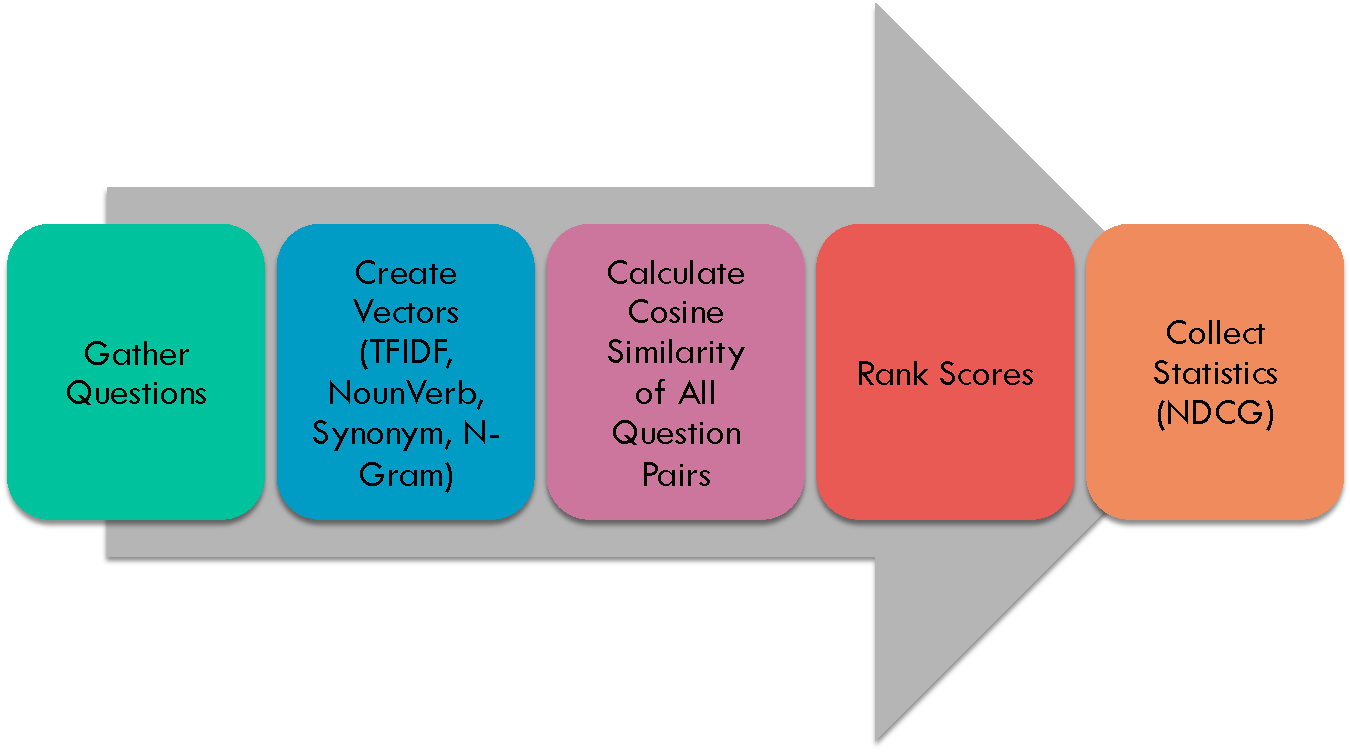
\includegraphics[width=1\columnwidth]{images/overall_structure.pdf}
\caption{The Overall Process of  Finding Similar Questions}
\label{fig:structure}
\end{figure}


\subsection{Data Collection}
StackExchange is a fast-growing network of 119 question and answer sites on diverse topics from software programming to cooking, photography to gaming. We selected two sub-sites from the StackExchange network, one is StackOverflow, which is the main site for programing questions, and has more than 700,000 questions. For our experiments, we collected all questions with tag Python, which has about 280,000 questions. The other sub-site we selected is English.StackExchange.com, which focuses on English questions regarding items like grammar or word usage. Since the number of the questions on this site is not large (35,600 in total) we used all the questions on this site.  

As all researchers in this domain know, datasets must be labelled in order to collect statistics regarding similarity and ranking. We chose to let the structure of the questions themselves contribute to this ranking. Many StackExchange contributors will provide links to other questions as part of their answer, i.e. ``This question was answered in this other thread. Check it out and see if it helps.” These links are stored by StackExchange as bidirectional edges between questions. So, if document A contains a link to document B, then a link exists between A and B, as well as B and A. We are aware that there likely exist questions that are similar but were not linked, and attempt to account for that by using only two relevance scores: a score of 1 indicates known similarity, whereas a score of 0 indicates unknown similarity. We utilize these scores in our NDCG statistics, discussed in Section X. As an additional precaution (and to limit experiment runtime), we disregarded collected questions that had no links. In total, there are 9291 questions in the Python dataset, 7693 in the English dataset, and 17,243 in the combined dataset. 

StackExchange provides REST style APIs which allowed us to gather for each question a title, a description (question body), linked questions, and a unique identifier. We used two specific API calls to collect the data:

1. /questions : This allowed us to get all the questions on the site. This method allows requesters to make fairly flexible queries across the entire corpus of questions on a site. For example, getting all questions asked in the the week of Jan 1st 2011 with scores of 10 or more is a single query with parameters sort=votes\&min=10\&fromdate=129384. The parameters we used in this experiment are: website, tag, start, pageSize  etc. 

2. /questions/{ids}/linked:  This call allowed us to procure questions which link to those questions identified in {ids}.  This method only considers questions that are linked within a site, and will never return questions from another StackExchange site. Two questions are considered "linked" when one question explicitly includes a hyperlink to the other question, there are no other heuristics.

There one final problem we met when collecting the data. To prevent malicious requests,  the server of StackExchange uses a time window to control the request number, like  100 requests every 15 minutes. So we needed to cut speed of our data collection program by forcing it to sleep for a designated number of seconds. The other strategy the server used to prevent malicious requests is that after some thousands of requests, the server will block the client IP. To combat this, we needed to change our physical location frequently to use new IP addresses.


\subsection{Tokenization (Data Cleaning)}
After data collection, it requires preprocessing. We consider one question as a document, and attempt to capture all of the alphanumeric words within the document. All non-alphanumeric characters (punctuation, spaces, etc.) were considered word separators. This means that compound words connected by a hyphen (`-’) and contractions (such as ``can’t”) are separated into two distinct words. During data cleaning, we also remove all hyperlinks because they contribute little to the message contained within the document, but take up much space in our indexes. For each document, we store each token and the number of occurrences within the document. This tokenization is the initial form of the vector. A term can be considered one dimension of that vector, while all terms with zero occurrences in a document have an assumed dimensional value of 0.


\subsection{Create Vectorizers}
As mentioned above, the contribution of our work is in the testing of the simple ideas proposed by researchers within their complex systems. We use their ideas in the formation of the vector and then use a single similarity metric (cosine) across all experiments to be sure that the vector is the only variant. We call these vector-definers `vectorizers’. We have three vectorizers: N-gram, synonym, and NounVerb. We use simple TF-IDF weighting on the original vector described in Section X as our baseline. TF indicates term frequency and IDF is inverse document frequency. 

\subsubsection{N-gram}
A compound noun is combined a sequence of two or more words that describe a single person, place, or thing. These kinds of words are unintentionally ignored in the bag-of-words vector model utilized by many systems. To solve this problem, we (and the authors of \cite{millar2006performance} before us) add N-grams to the original vector. N-grams are phrases taken directly from the document of length N.  To generate the N-gram vector for a document, each consecutive set of terms N terms is considered an additional dimension in the vector space. Figure X depicts the bag of words for the phrase ``for loop in python” with added N-grams (N=2).

The weight of N-gram dimension in the vector space is the TFIDF value of the N-gram (calculated the same way as individual tokens). We conducted experiments for N=2 and N=3. 

\subsubsection{Synonym}
Often there exists many words to express the same sentiment and question-askers might use any of these words when composing their questions. Therefore, the authors of \cite{liu2009searching} propose adding synonyms for each word in the vector. We do this using Wordnet in NLTK (Natural Language Toolkit) \cite{NLTK}. This tool finds similarity between words and provides the synonyms of a word. Some synonyms often fail to convey semantic similarity, but we claim that it is worth trying. Figure X shows the bag of words after the phrase ``for loop in python” exits the Synonym vectorizer. 

The weight of each added synonym is the TF-IDF value of the original word (to which the new word is a synonym) multiplied by the Wordnet supplied similarity  score (in the range of 0-1) between the two words. So, a synonym that is very similar to the original word would have a weight very close to the original word, while a synonym that is only marginally similar to the original word will have a very small weight.

We conducted experiments with 1 added synonym and 2 added synonyms. We collected preliminary results for 3 synonyms, but due to poor results and long runtimes, we discontinued those experiments.

\subsubsection{Weighting nouns and verb}
The authors of \cite{wang2009syntactic} suggest weighting nouns and verbs more heavily than other words because they contribute more to the meaning of the sentence. The authors believe that different parts of the sentence have varying importance, and the nouns and verbs are considered to be more important than other types of terms such as articles, adjectives or adverbs. Hence, we boost up the nodes of verb and noun phrases, to show their higher priority over other ordinary ones. The authors of \cite{wang2009syntactic} suggest weighting non-nouns and non-verbs normally (for us that means TFIDF), but boosting the weight of nouns and verbs by a factor of 1.2 (TFIDF*1.2). For tagging nouns and verbs, we use NLTK tagging.

\subsection{Calculate Similarity}
Though the composition of the vectors is variable, it is important for purposes of comparison that the similarity function remain static. We use cosine to determine the similarity between two documents. Cosine similarity is a measure of the angle between two vectors. Two identical vectors will have a cosine score of 1. The equation is described below.

We determine the cosine scores between each document and every other document in the dataset. We then rank (sort) those scores into descending order. Each of these document orderings is called a ranking. 

\section{Result and Analysis}
\subsection{Statistics \& Measures}
We collected several statistics in order to determine which vectorizers, in combination with our cosine similarity function, will provide the best-ranked list of similar questions. 
\begin{enumerate}[noitemsep]
	\item NDCG (Normalized Discounted Cumulative Gain) - This is a statistic used to evaluate rankings. Simply, each document is labeled with a relevance score. Higher scores indicate higher relevance. Then, based on the relevance score and the rank of each result, we accumulate the total score such that higher ranked results contribute more to the final score than lower-ranked results. Finally, we normalize the score by dividing by the best possible ranking to find the final NDCG. 
Generally relevance scores are all greater than zero (i.e. 3=Great, 2=Average, 1=Terrible). However, since we do not have the whole ground truth (two documents might be similar, but no one chose to link them), we chose relevance scores of 1=Similar (Linked), 0=Unknown. This ensures that documents of unknown similarity do not contribute to NDCG scores. This does not fully mediate the issue of the missing similarity, but we believe it lessens the negative effects considerably.
Of the NDCG scores, we collected the mean, median, mode, standard deviation, max value, and min value.
	\item TopRank - This is a statistic of our invention that simply keeps track of the rank of the first similar document in a ranking. For example, if the first result returned by a ranking had no link to the query question, but the second result did have a link to the query, the TopRank for that ranking would be 2. Of the TopRank scores, we collected the mean, median, mode, standard deviation, max value, and min value.
	\item Percent@Rank1 - This is the percentage of rankings that returned a linked result in the first position in the ranking.
\end{enumerate}

\subsection{Experiments}
In sum, we ran approximately 65 experiments to determine how the various methods of representing questions performed stacked up against one another. We tested each vectorizer (NGram 2, NGram 3, NounVerb, Synonym 1, Synonym 2, and the baseline TFIDF) against each each of the three datasets (Python, English, and Combined Python+English), and each of the three question scopes (question title only, question body only, question title + body). 
Note that the above-mentioned list only equates to 54 experiments (6 vectorizers x 3 datasets x 3 scopes). We additionally ran preliminary experiments for Synonym 3, but due to its extremely low performance and long runtimes (about 8 hours each), we ceased running experiments of that type.

\subsection{Result}
Of the three question scopes (question title only, question body only, question title + body), we found (not surprisingly) that title+body performed best across all vectorizers and all datasets. Figure \ref{fig:toprankmedians} shows the median TopRank scores for each dataset, vectorizer, and scope. The Title+Body scope provided median TopRanks three times better (on average) than titles alone. For this reason, the remainder of results discussed will be for the Title+Body question scope.

\begin{figure}[!htb]
\centering
\minipage{0.32\textwidth}
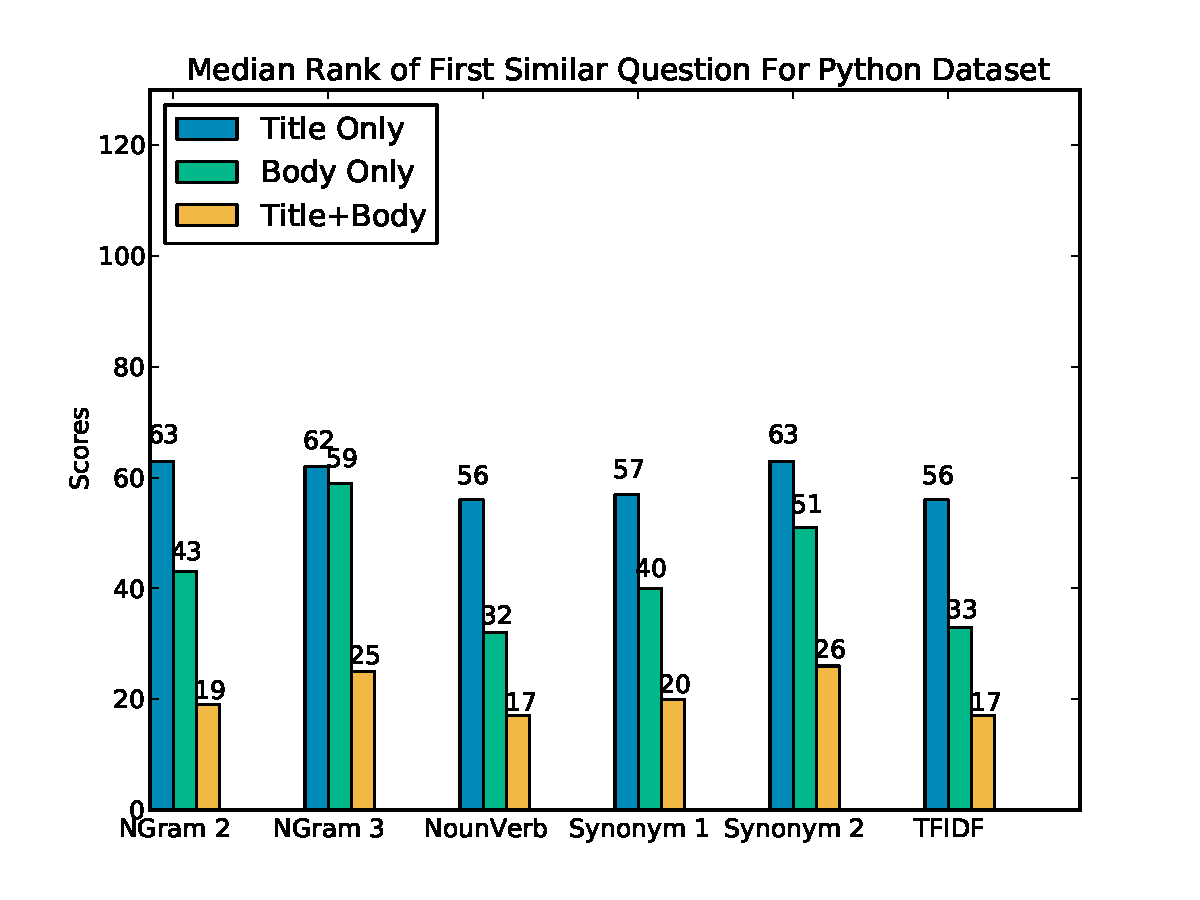
\includegraphics[width=1.1\linewidth]{images/Python_all-toprank-medians_plot.pdf}
\endminipage\hfill
\minipage{0.32\textwidth}
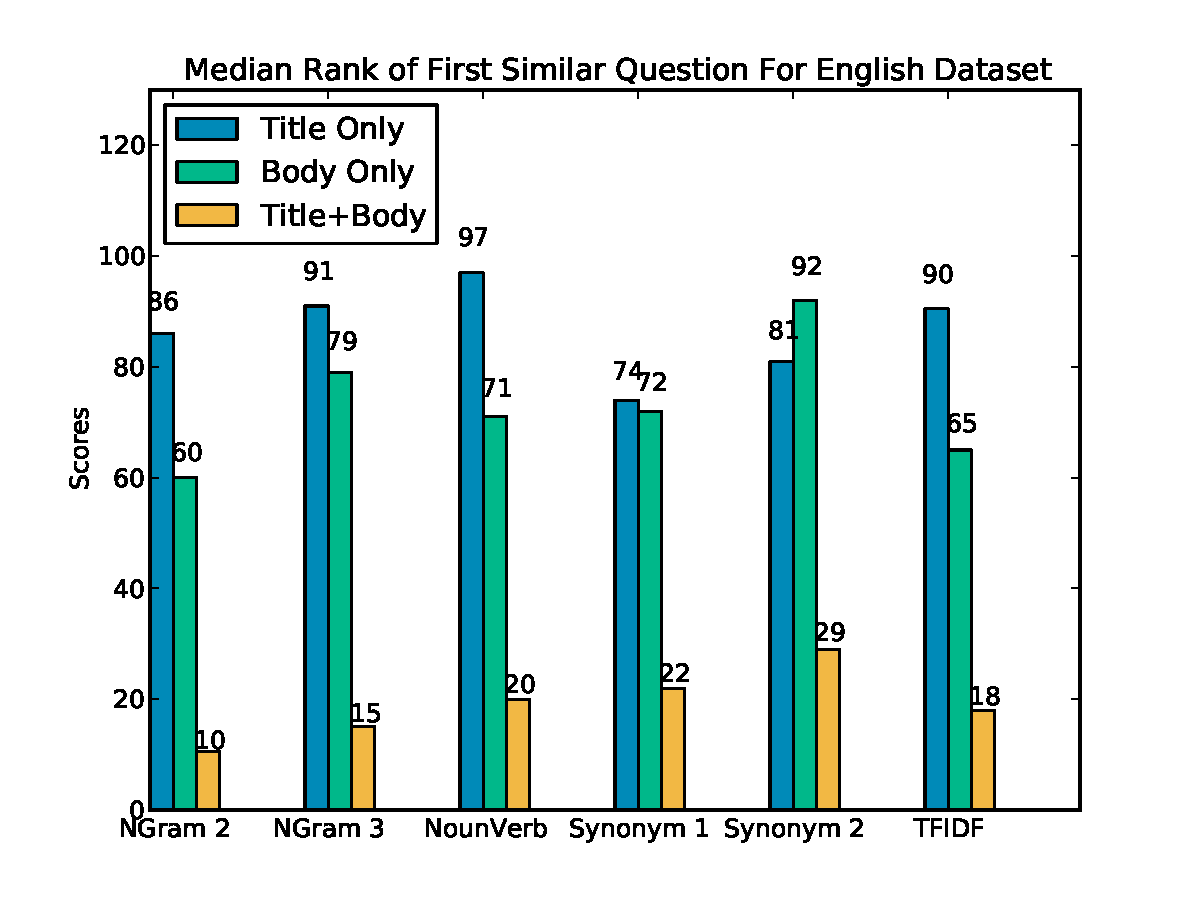
\includegraphics[width=1.1\linewidth]{images/English_all-toprank-medians_plot.pdf}
\endminipage\hfill
\minipage{0.32\textwidth}%
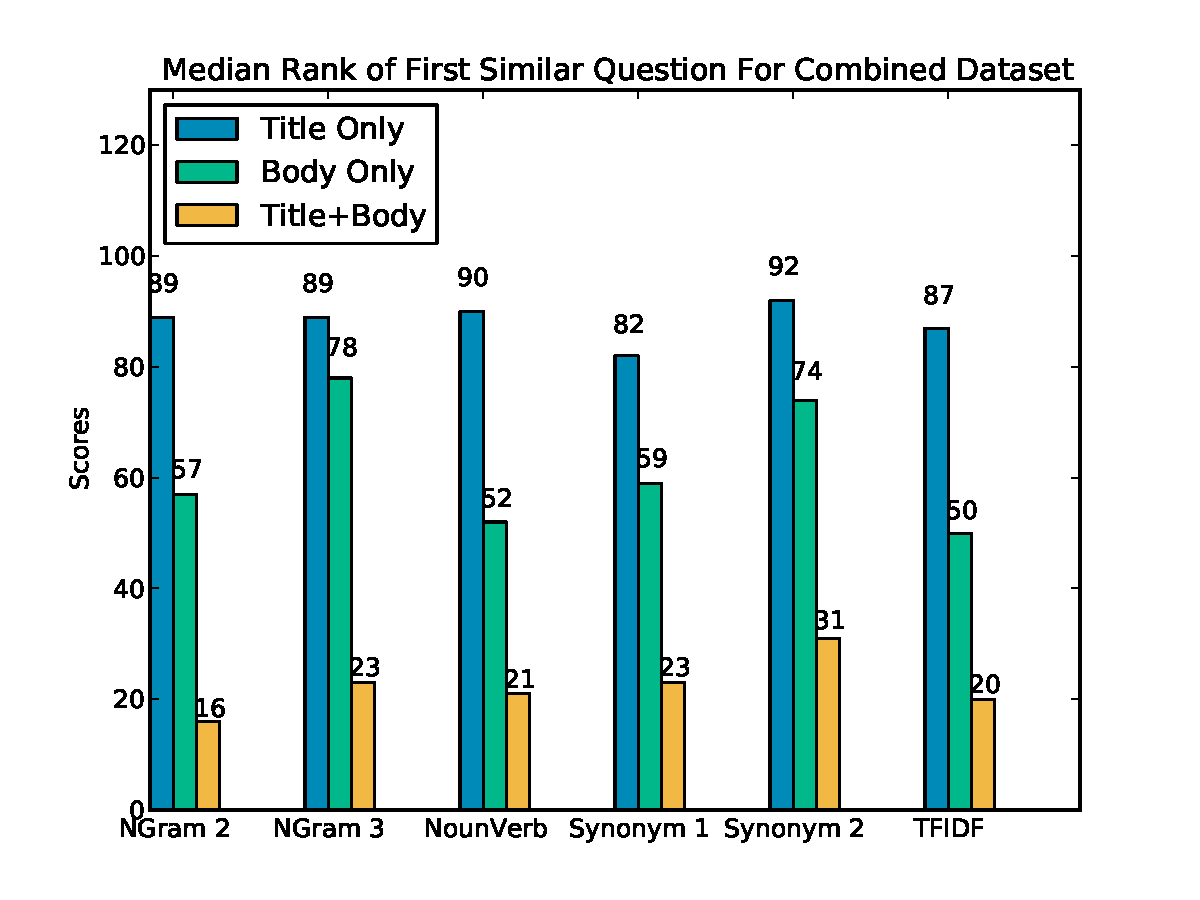
\includegraphics[width=1.1\linewidth]{images/Combined_all-toprank-medians_plot.pdf}

\endminipage

\caption{Median TopRank scores across datasets, vectorizers, and scopes.}
\label{fig:toprankmedians}
\centering
\end{figure}



We were surprised to find that only one vectorizer (N-Gram 2) outperformed our baseline TFIDF in a majority of cases. Figure \ref{fig:allmeans} shows Mean NDCG scores with standard deviation bars for each vectorizer and dataset (higher values indicate better results). Though all vectorizers appear to behave similarly, the NGram 2 vectorizer (N-Grams where N=2) performed statistically significantly better in terms of NDCG than all other vectorizers (p<.01) for the combined dataset.

\begin{figure}[h]
\centering
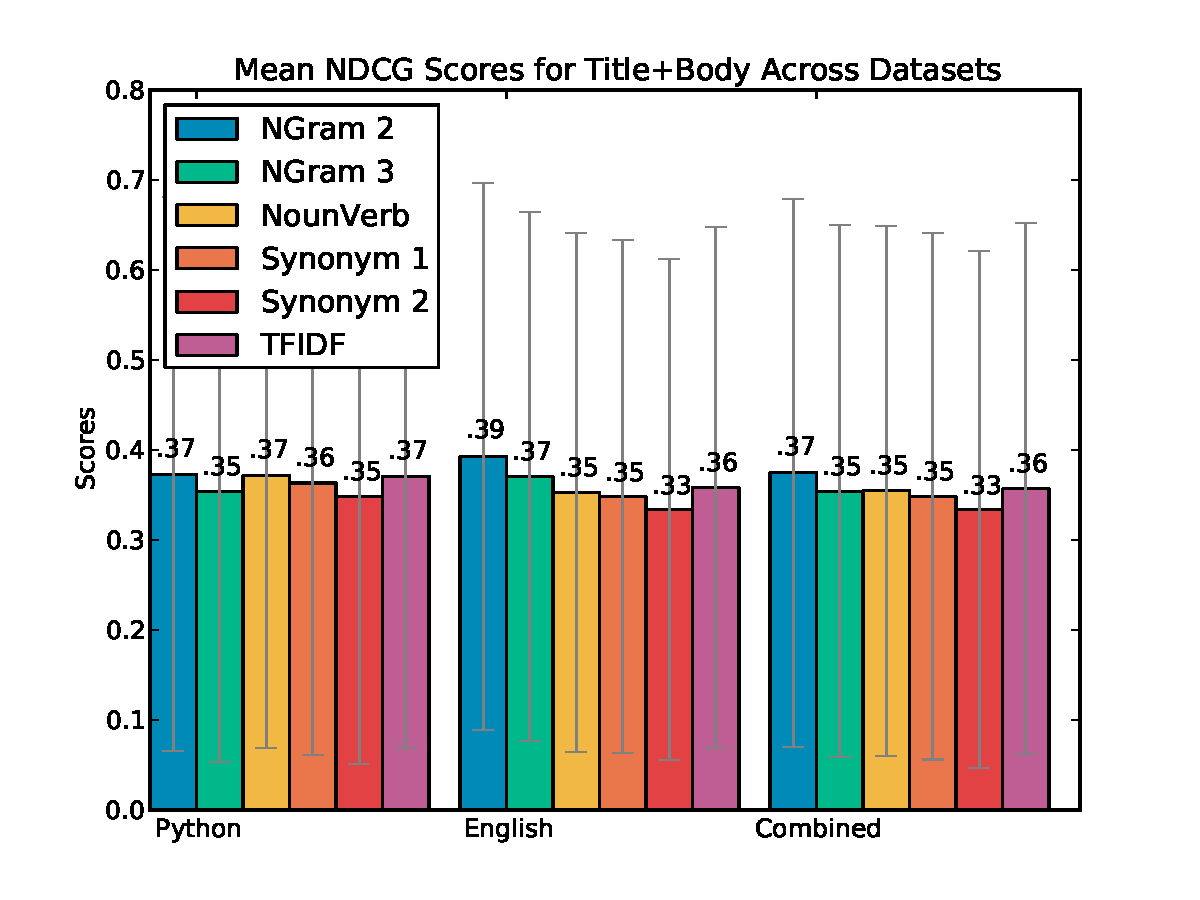
\includegraphics[width=1\columnwidth]{images/all-means-by-dataset_plot.pdf}
\caption{Means and standard deviations of NDCG results across all datasets and vectorizers for Title+Body scope.}
\label{fig:allmeans}
\end{figure}

	
Figure X shows the Percent@Rank1 for each vectorizer and dataset (higher values indicate better results). In terms of Percent@Rank1, both NGram vectorizers tested (2 and 3) performed better than the baseline TFIDF across all datasets. 

\begin{figure}[h]
\centering
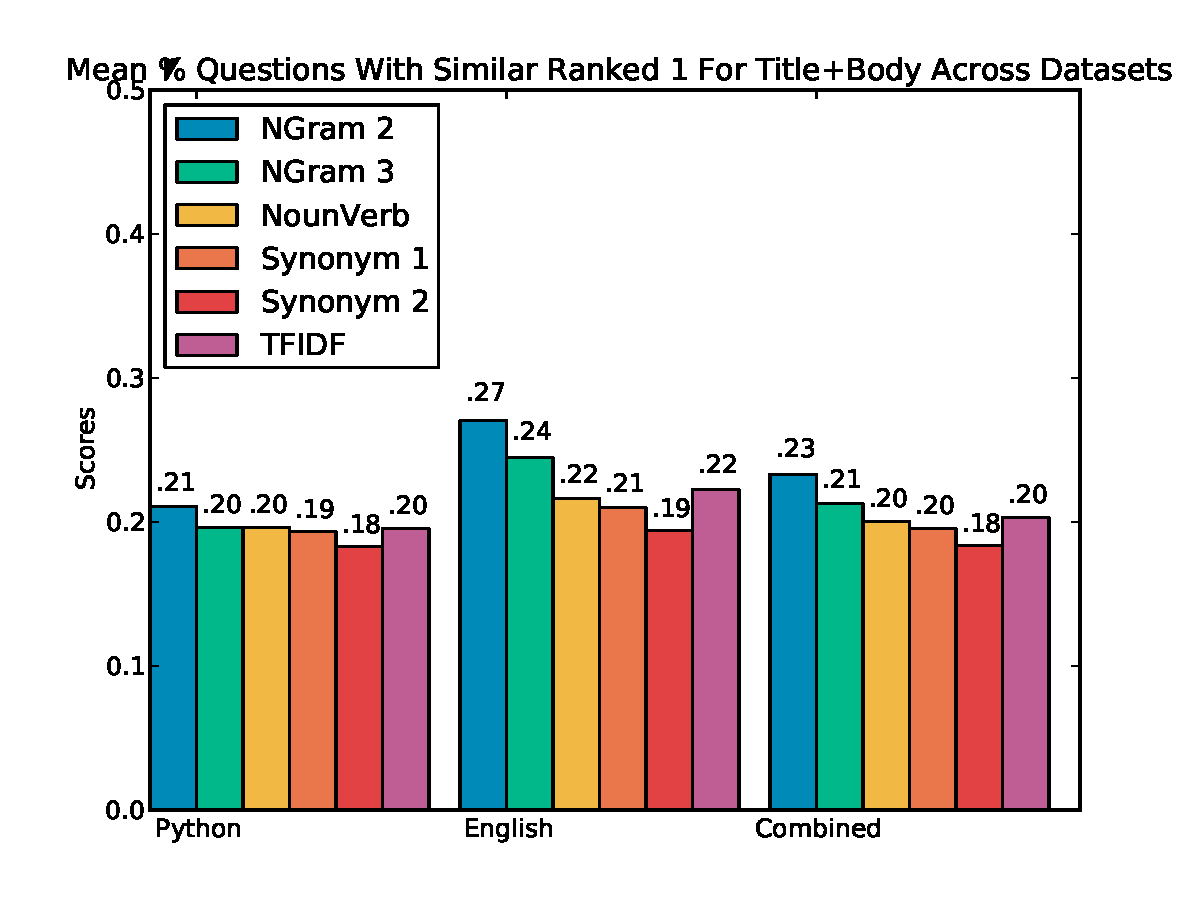
\includegraphics[width=1\columnwidth]{images/all-percent@rank1-by-dataset_plot.pdf}
\caption{Means and standard deviations of NDCG results across all datasets and vectorizers for Title+Body scope.}
\label{fig:allmeans}
\end{figure}
	
Figure X shows the median TopRank for each vectorizer and dataset (lower values indicate better results). Though the mean TopRank scores show few significant differences, the medians shown in Figure X indicate that more results from the NGram 2 vectorizer would be found satisfactory by users.

$[all-median-topRanks-by-dataset_plot]$

	Across all statistics, we found that the NounVerb vectorizer performed about as well as TFIDF for all datasets and question scopes (no statistically significant differences). Though this may have increased performance for \cite{wang2009syntactic}, increased weighting for nouns and verbs  made no difference in our system.


\section{Conclusion}
In sum, the contribution of this work is that many of the ideas proposed by researchers to improve similarity results of questions in community-based Q\&A systems make little or no significant improvement over simple TFIDF weighting. It appears to us that the further the vector deviated from the original bag-of-words for the document, the worse the system performed. Adding synonyms decreased performance, but increasing the weights of nouns and verbs made little difference. 

The one exception to the generalization that deviations from the bag-of-words model decrease performance is the NGram 2 vectorizer, which, we argue, captures more of the essence of the original document than basic bag-of-words tokenization. Thus, it performed better than simple TFIDF. NGram 3 may have captured too much of the structure of the original document, and thus stylistic differences in writing by different authors caused NGram 3 to not perform to the quality of NGram 2.
%\end{document}  % This is where a `short' article might terminate


%
% The following two commands are all you need in the
% initial runs of your .tex file to
% produce the bibliography for the citations in your paper.
\bibliographystyle{abbrv}
\bibliography{sigproc}  % sigproc.bib is the name of the Bibliography in this case
% You must have a proper ".bib" file
%  and remember to run:
% latex bibtex latex latex
% to resolve all references
%
% ACM needs 'a single self-contained file'!
%
\end{document}


